\providecommand{\main}{../../main}
\documentclass[../../main/main.tex]{subfiles}


\begin{document}


\section{Experimental apparatus}
\label{sec:apparatus}
In this Section we describe the experimental apparatus designed for the experience, focusing in particular to the new improvements made with respect to the previous years iterations. The structure of the setup is characterised by its modularity. In fact, we can distinguish several connected sections, in particular:
\begin{itemize}
    \item a \textbf{radioactive source} of \( {}^{241}\mathrm{Am} \), with the active material inside an aluminium cylinder. The overall structure of this piece is inlaid in a 3d-printed support;
    \item a \textbf{vacuum system}, including a vacuum chamber, a pumping station to reach the vacuum condition and two vacuum gauges to keep track of the internal pressure of the chamber;
    \item a \textbf{mechanical system}, including a step motor through which the support of the source is rotated. This is connected to an Arduino shield tower and to a computer, through which the step position can be regulated;
    \item a set of \textbf{thin foils} of different materials, such as gold and tin, on which the \( \alpha \) particles can scatter;
    \item a partially depleted \textbf{Silicon Surface Barrier (SSB) detector}, connected to a NIM module electronics chain and then to a PicoScope digital oscilloscope acting as digitizer, in order to sample the waveforms of the candidate \( \alpha \) signals;
    \item an \textbf{ALice PIxel DEtector (ALPIDE)}, whose acquisition is managed by a Field Programmable Gate Array (FPGA) with a dedicated firmware;
\end{itemize}
Hereafter we describe each of these components in detail, starting from the inner core of the apparatus, namely the vacuum system, and finally coming to the two independent detection systems with SSB and ALPIDE detectors, respectively. In addition, we also discuss about a configuration of the Local Network Area in our apparatus in order to improve the capabilities of remote control of the acquisitions.



\subsection{Vacuum system}

\paragraph{Vacuum chamber}
The core component of the vacuum system, in which the scattering process takes place, is the vacuum chamber. It has a cylindrical form and its internal diameter is of about \( 22 \ \si{cm} \). It has several gateways on its side surface, where the so-called feedthroughs can be placed to transfer all the electronic signals outside the chamber. The whole chamber is showed in \figref{fig:vacuum_chamber_photo}.


\paragraph{Pumping station}
One of the gateways is dedicated to the connection to the pumping station Pfeiffer Vacuum HiCube-80, showed in \figref{fig:vacuum_station_photo} and versatile for all high and ultrahigh vacuum applications \cite{pfeiffer}. The latter is composed of a diaphragm pump and a turbomolecular pump. Their operations during their working are automated: firstly, the diaphragm pump will produce low vacuum, then the turbomolecular will slowly reach its regime and produce the high vacuum needed. To lower the stress to the turbomolecular pump, two pipes in the middle of the station and the chamber are inserted, with different magnitudes of conductance. The higher conductance pipe has an on-off valve type, while the low conductance one has a variable valve to tune its conductance. These are showed in \figref{fig:vacuum_valves}.


\paragraph{Gauges, valves and working point}
When making the vacuum, two independent gauges monitor the pressure in the vacuum system. The first one, namely a \textbf{Penning} gauge, is placed in the chamber and it gives information on the internal pressure of the apparatus. The second one, namely a \textbf{Pirani} gauge, is placed just after the turbomolecular pump in order to signal an eventual stress to the turbine when the variable valve impedance is excessive. Moreover, a third variable valve is placed right before the turbomolecular pump in order to break the vacuum slowly and preserve sensible devices inside the chamber, such as the target foils.

A complete setup of the vacuum valves is showed in \figref{fig:vacuum_valves}. Through this whole vacuum setup, it is possible to reach the working point pressure for this experiment:
\begin{equation}
    p
    =
    (9.0 \pm 0.2) \cdot 10^{-5} \ \si{mbar}
    \quad .
    \label{eq:vacuum_pressure}
\end{equation}
This is sufficient to perform a scattering experiment with the required precision of measurements. In fact, the loss of energy due to the residual molecules of air in the chamber can be reasonably neglected with respect to the losses due to other factors, treated in the following Subsections.

\begin{figure*}[h]
    \begin{minipage}[c]{0.33\linewidth}
        \vspace{0pt}
        \centering
        \subfloat[Vacuum chamber]{%
            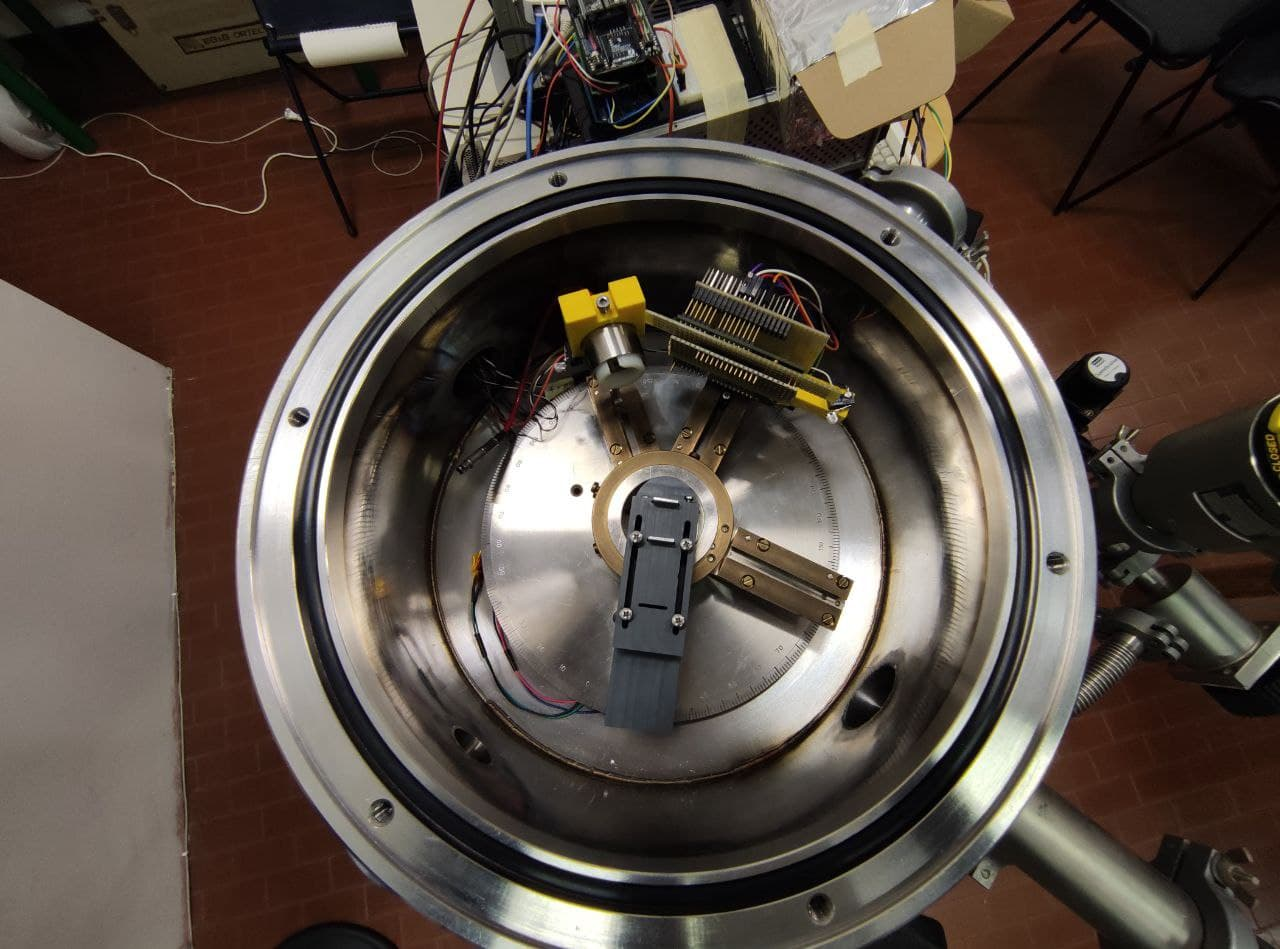
\includegraphics[width=\textwidth]{../sections/02/images/apparatus/vacuum_chamber.jpg}%
            \label{fig:vacuum_chamber_photo}%
        }%
    \end{minipage}%
    \hfill%
    \begin{minipage}[c]{0.33\linewidth}
        \vspace{0pt}
        \centering
        \subfloat[Pumping station]{%
            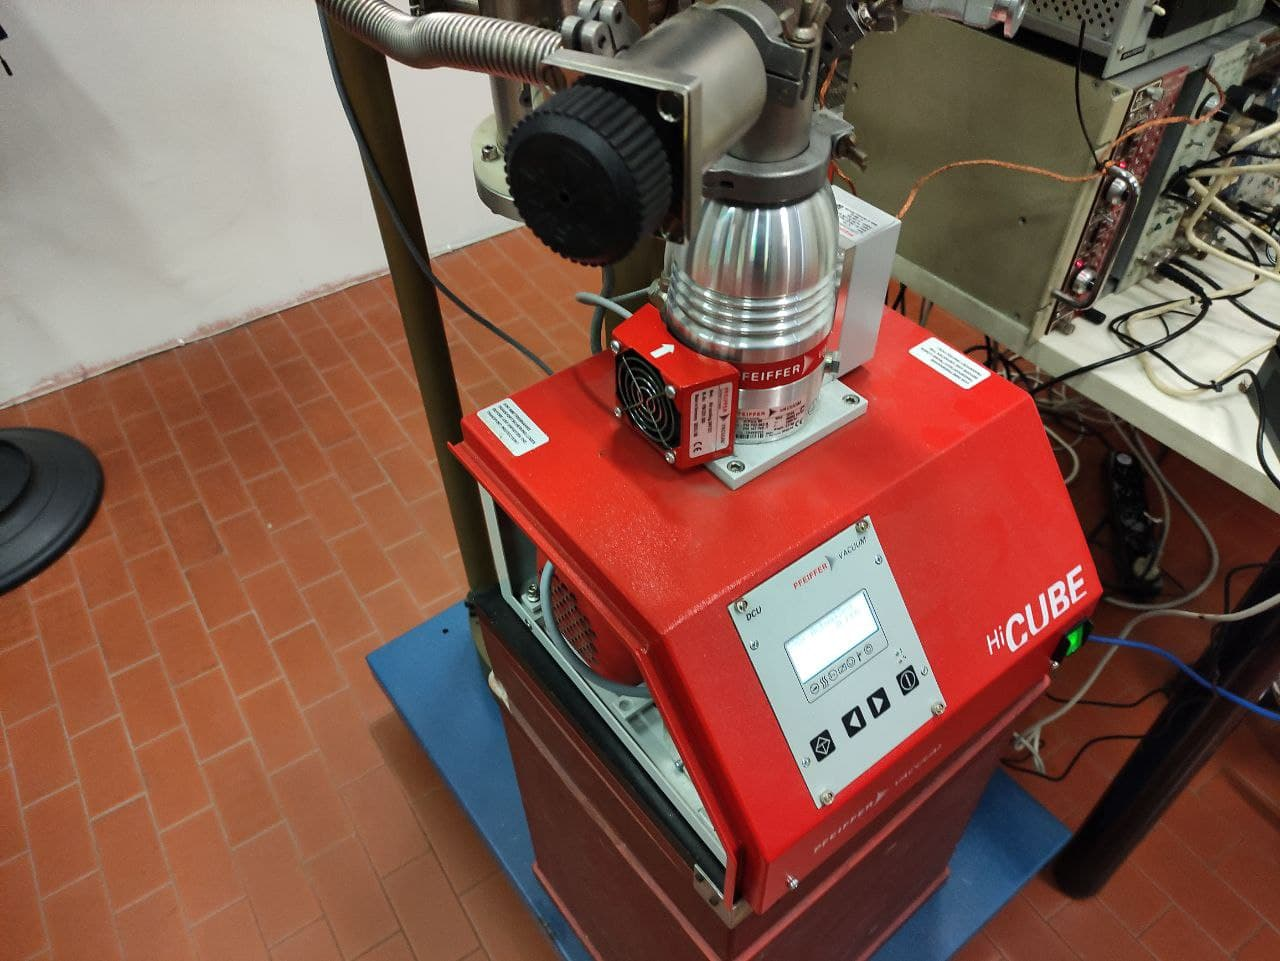
\includegraphics[width=\textwidth]{../sections/02/images/apparatus/pumping_station.jpg}%
            \label{fig:vacuum_station_photo}%
        }%
    \end{minipage}%
    \hfill%
    \begin{minipage}[c]{0.33\linewidth}
        \vspace{0pt}
        \centering
        \subfloat[Vacuum valves setup]{%
            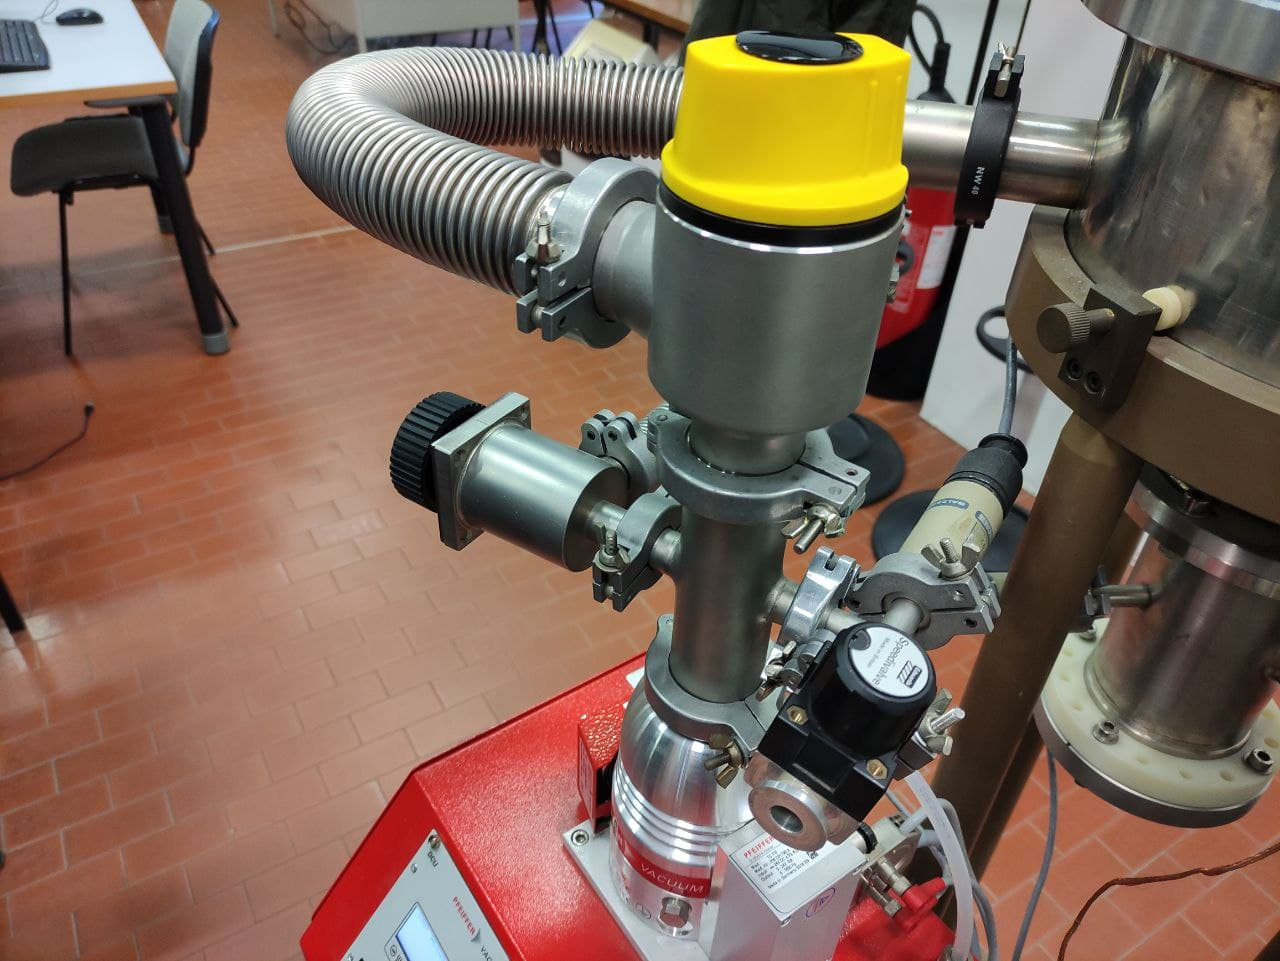
\includegraphics[width=\textwidth]{../sections/02/images/apparatus/vacuum_valves.jpg}%
            \label{fig:vacuum_valves}%
        }
    \end{minipage}%
    \label{fig:vacuum_components}
    \caption{Vacuum chamber employed for the experiment in \textbf{\ref{fig:vacuum_chamber_photo}} and pumping station Pfeiffer Vacuum HiCube-80 in \textbf{\ref{fig:vacuum_station_photo}}. In \textbf{\ref{fig:vacuum_valves}}, the whole vacuum valves setup.}
\end{figure*}



\subsection{Mechanical system}

\paragraph{Step motor}
Again, we start from the core component of this section of apparatus, namely the step motor, showed in \figref{fig:mechanical_step_motor}. It is hidden at the very bottom of the vacuum chamber and it allows to modify the angle of the source beam direction with respect to the detectors positions. More in particular, the step motor is a 4-cable type with two sets of active coils, through which its revolution is divided into 400 steps. Therefore, the angular interval covered in a single step rotation is equal to:
\begin{equation}
    \Delta \theta_{\mathrm{step}}
    =
    (0.9 \pm 5\%) \ \si{deg}
    \quad .
    \label{eq:mechanical_step}
\end{equation}
In order to control the step motor from a computer, an Arduino microcontroller is exploited. In particular, this part includes also two overlying shields, designed in a previous iteration of the experience and translating the Arduino digital signals in actual impulses for the motor. Moreover, the shields are connected to two microswitches placed at the edges of the detection system to define the angular boundaries needed to perform an angular calibration of the motor. One of them is showed in \figref{fig:mechanical_microswitch}.


\paragraph{Source support and collimators}
A 3d-printed plastic support for the radioactive source is directly connected to the shaft of the motor, so that it can rigidly rotate with the motor itself. This piece is showed in FIG. \figref{fig:mechanical_source_support}, where we can be observe its composite shape with two grooves. The ladders are designed to securely accommodate the two collimation targets. Moreover, on its final part, in front of the last collimator, there are two threads on which the scattering foil can be locked through two screws.

Concerning the collimators, these are nothing more than aluminium targets with an engraved groove, whose width \( c_{1} \), height \( c_{2} \) and thickness \( c_{3} \) are listed in \tabref{tab:mechanics_collimator_dimensions} along with the distance \( d_{\mathrm{cc}} \) between the two collimators. A picture of a sample of this component is showed in \figref{fig:mechanical_collimators}.

\begin{table}[h]
    \centering
    \begin{tabular}{ccc}
        \toprule
        \textbf{Dimension}  &   \textbf{Symbol} &   \textbf{Length [mm]} \\
        \colrule
        Groove width    &   \( c_{1} \) &   \( 4.0 \)   \\
        Groove height    &   \( c_{2} \) &   \( 7.0 \)   \\
        Groove thickness    &   \( c_{3} \) &   \( 1.3 \)   \\
        Groove-Groove distance  &   \( d_{\mathrm{cc}} \) &   \( 20.0 \)   \\
        \botrule
    \end{tabular}
    \caption{Relevant physical dimensions for the two collimation targets, in particular for their grooves and their reciprocal distances, which are of crucial importance for a correct modelling of the apparatus.}
    \label{tab:mechanics_collimator_dimensions}
\end{table}


\paragraph{Detectors supports}
The SSB detector support is made of a metallic frame and a plastic structure in which one of the microswitches is fixed. The metallic frame consists in a base connected to a rail over the base of the vacuum chamber, and a hollow cylinder housing the detector. The latter is collimated with a metallic annular target, whose groove diameter length is \( 4 \ \si{mm} \). The latter is necessary to perform finer angular measurements for a fixed position. The overall support is showed in \figref{fig:mechanical_ssb_support}.

On the other hand, the ALPIDE support is a simple 3d-printed base inserted in an another rail of the chamber. On this polymer structure, a PCB is fixed and some pins are soldered on it for the needed ALPIDE shield connections. Again, the structure of the support is showed in \figref{fig:mechanical_alpide_support}, where we can also observe the second last microswitch fixed on the plastic base.

The distances of both the supports from the centre of rotation of the motor are measured indirectly through angular measurements with the aim of a laser. It is possible to do this with high precision since the dimensions of ALPIDE and SSB detectors supports are known with a negligible uncertainty. So, given the angular extension \( \Delta \theta \) of the support of the SSB or of ALPIDE detector and their length \( \ell \), we can extract the distance \( d \) with simple calculations:
\begin{equation}
    d
    =
    \frac{\ell}{2} \operatorname{ctan}^{-1}\qty(\frac{\Delta \theta}{2})
    \quad .
\end{equation}
We report the results for the distances from the supports in \tabref{tab:mechanics_support_distances}.

\begin{table}[!h]
    \centering
    \begin{tabular}{cc}
        \toprule
        \textbf{Component}  &   \textbf{\boldmath\( d \) [mm]}   \\
        \colrule
        ALPIDE detector & \( 78.6 \pm 0.7 \)    \\
        SSB detector    & \( 92   \pm 1   \)    \\
        \botrule
    \end{tabular}
    \caption{Distances of the two detectors with respect to the centre of rotation of the motor, coinciding with the centre of the vacuum chamber.}
    \label{tab:mechanics_support_distances}
\end{table}


\begin{figure*}[h]
    \begin{minipage}[c]{0.33\linewidth}
        \vspace{0pt}
        \centering
        \subfloat[Step motor]{%
            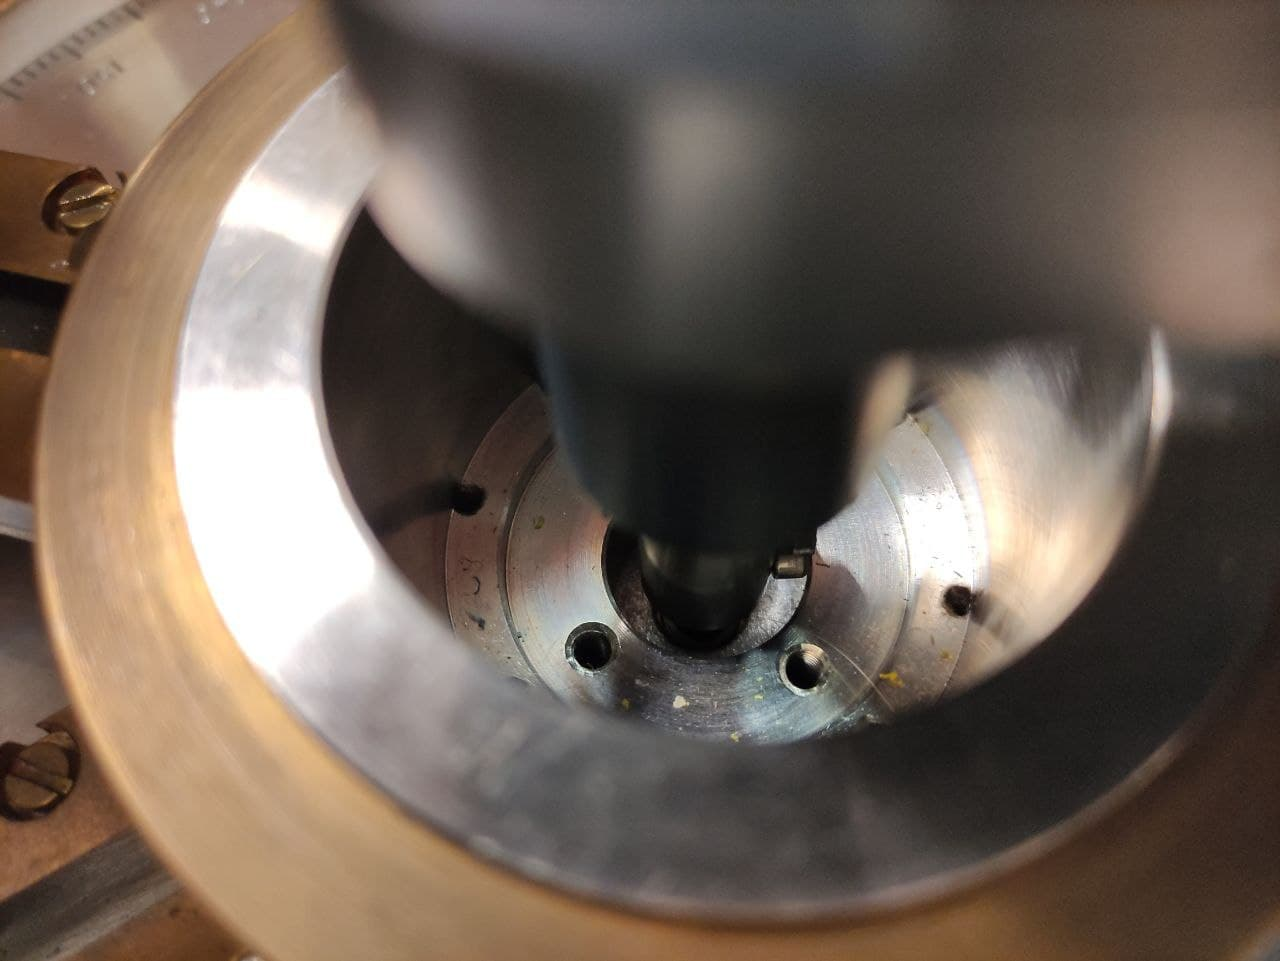
\includegraphics[width=\textwidth]{../sections/02/images/apparatus/step_motor.jpg}%
            \label{fig:mechanical_step_motor}%
        }%
    \end{minipage}%
    \hfill%
    \begin{minipage}[c]{0.33\linewidth}
        \vspace{0pt}
        \centering
        \subfloat[Source support]{%
            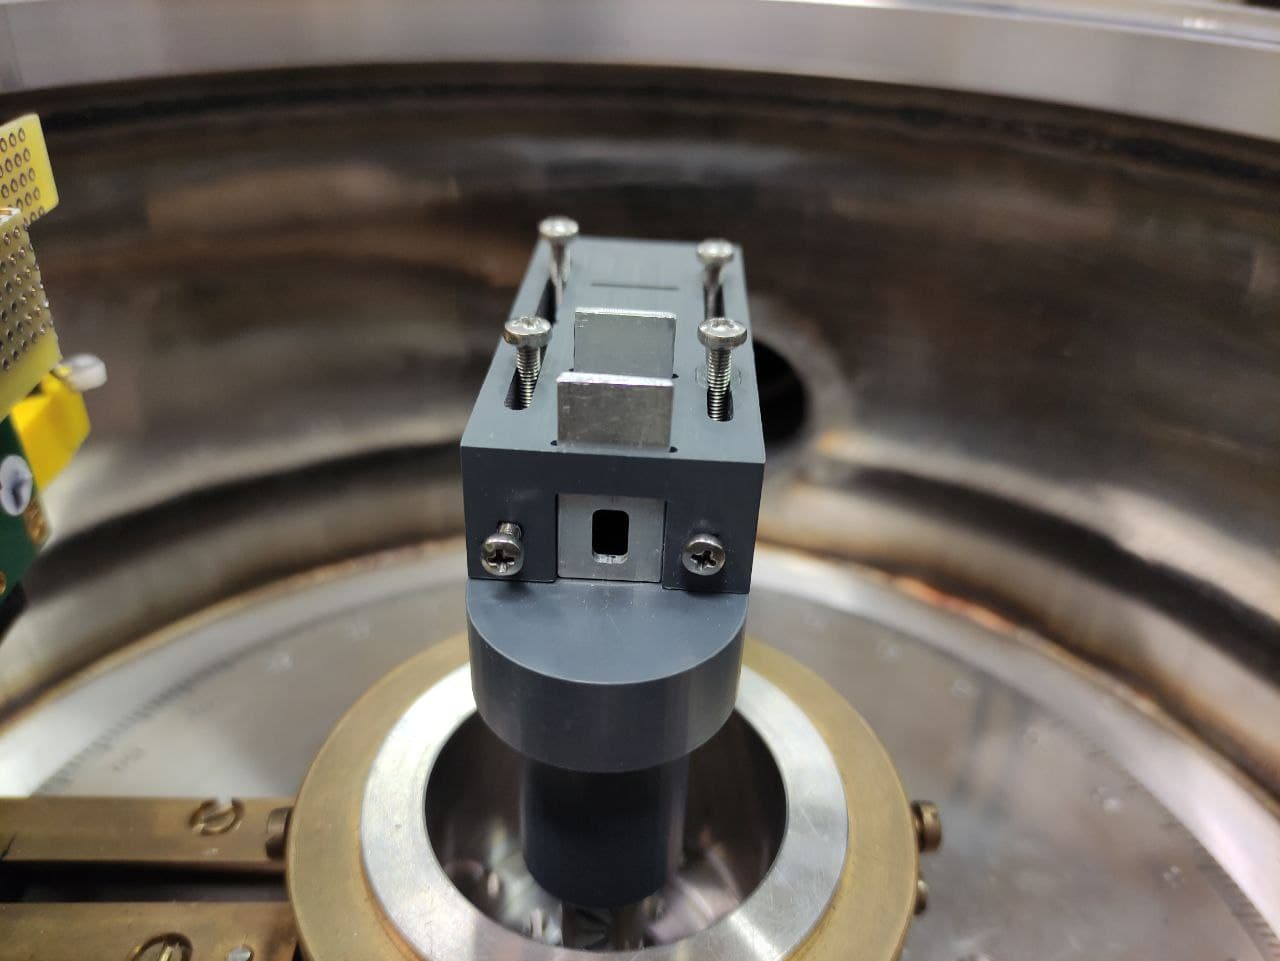
\includegraphics[width=\textwidth]{../sections/02/images/apparatus/source_support.jpg}%
            \label{fig:mechanical_source_support}%
        }%
    \end{minipage}%
    \hfill%
    \begin{minipage}[c]{0.33\linewidth}
        \vspace{0pt}
        \centering
        \subfloat[Microswitch]{%
            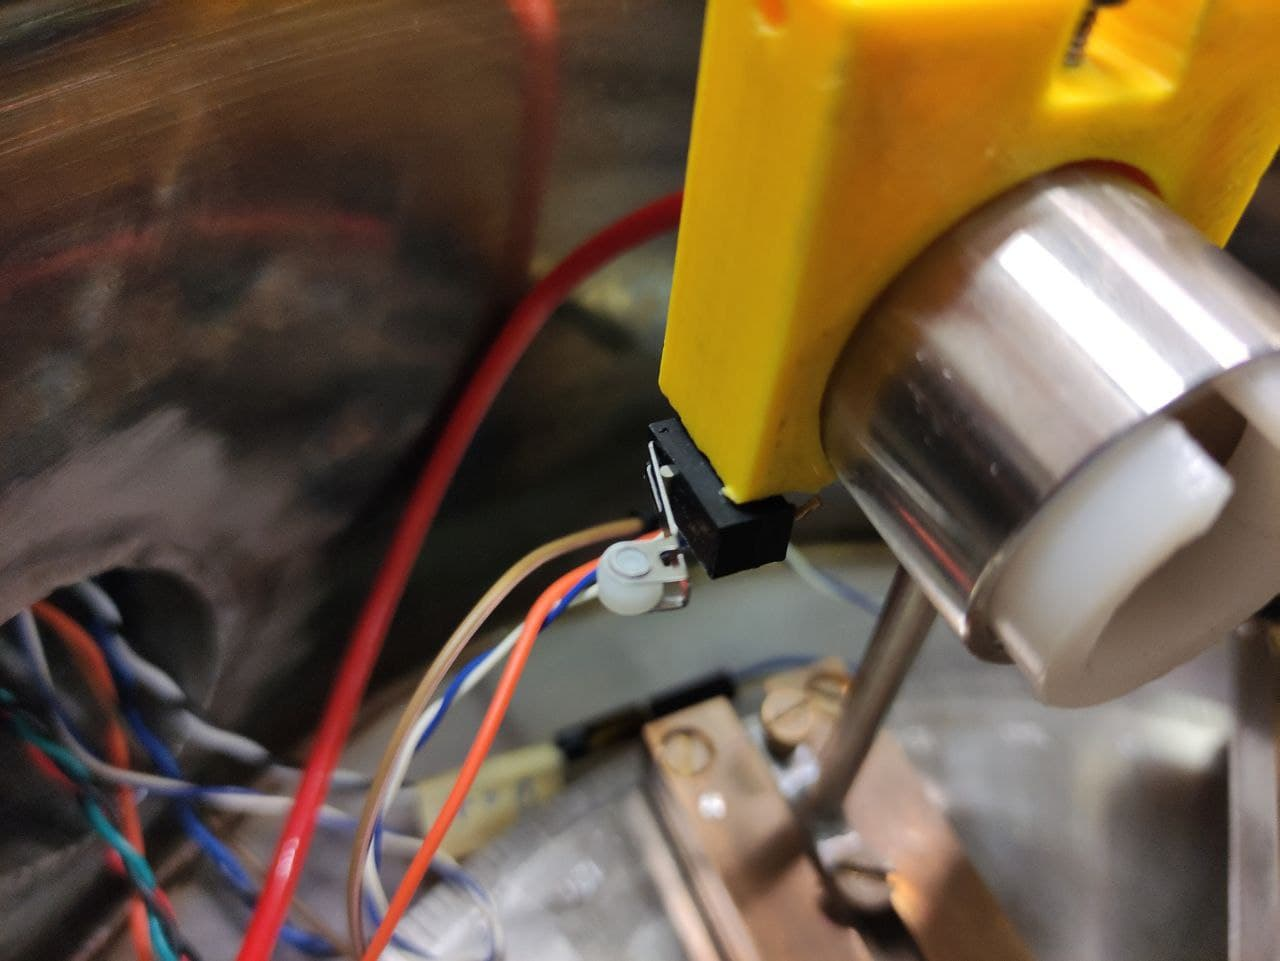
\includegraphics[width=\textwidth]{../sections/02/images/apparatus/microswitch.jpg}%
            \label{fig:mechanical_microswitch}%
        }%
    \end{minipage}%

    \begin{minipage}[c]{0.33\linewidth}
        \vspace{0pt}
        \centering
        \subfloat[Beam collimators]{%
            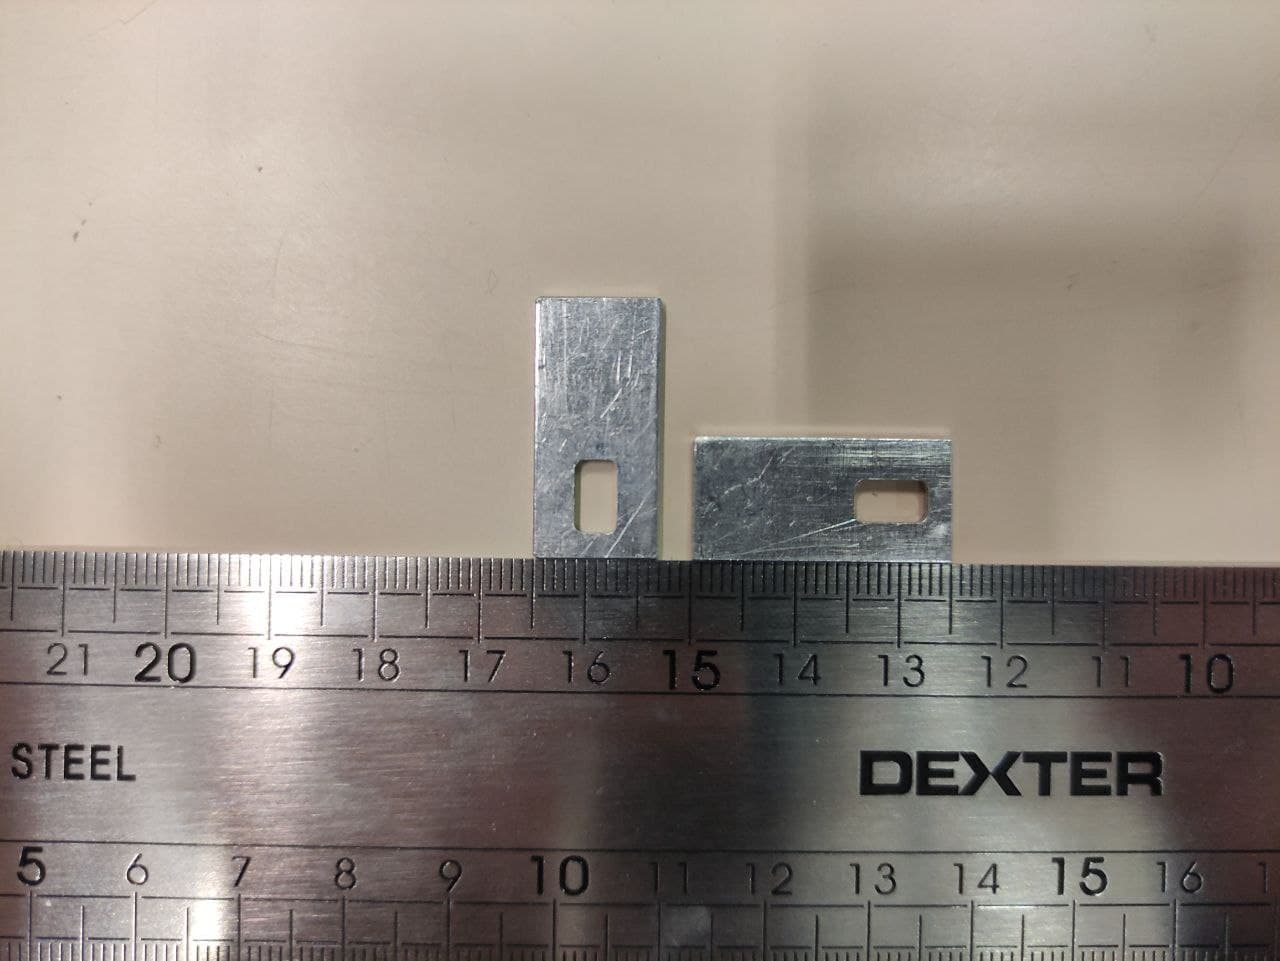
\includegraphics[width=\textwidth]{../sections/02/images/apparatus/collimators.jpg}%
            \label{fig:mechanical_collimators}%
        }%
    \end{minipage}%
    \hfill%
    \begin{minipage}[c]{0.33\linewidth}
        \vspace{0pt}
        \centering
        \subfloat[SSB detector support]{%
            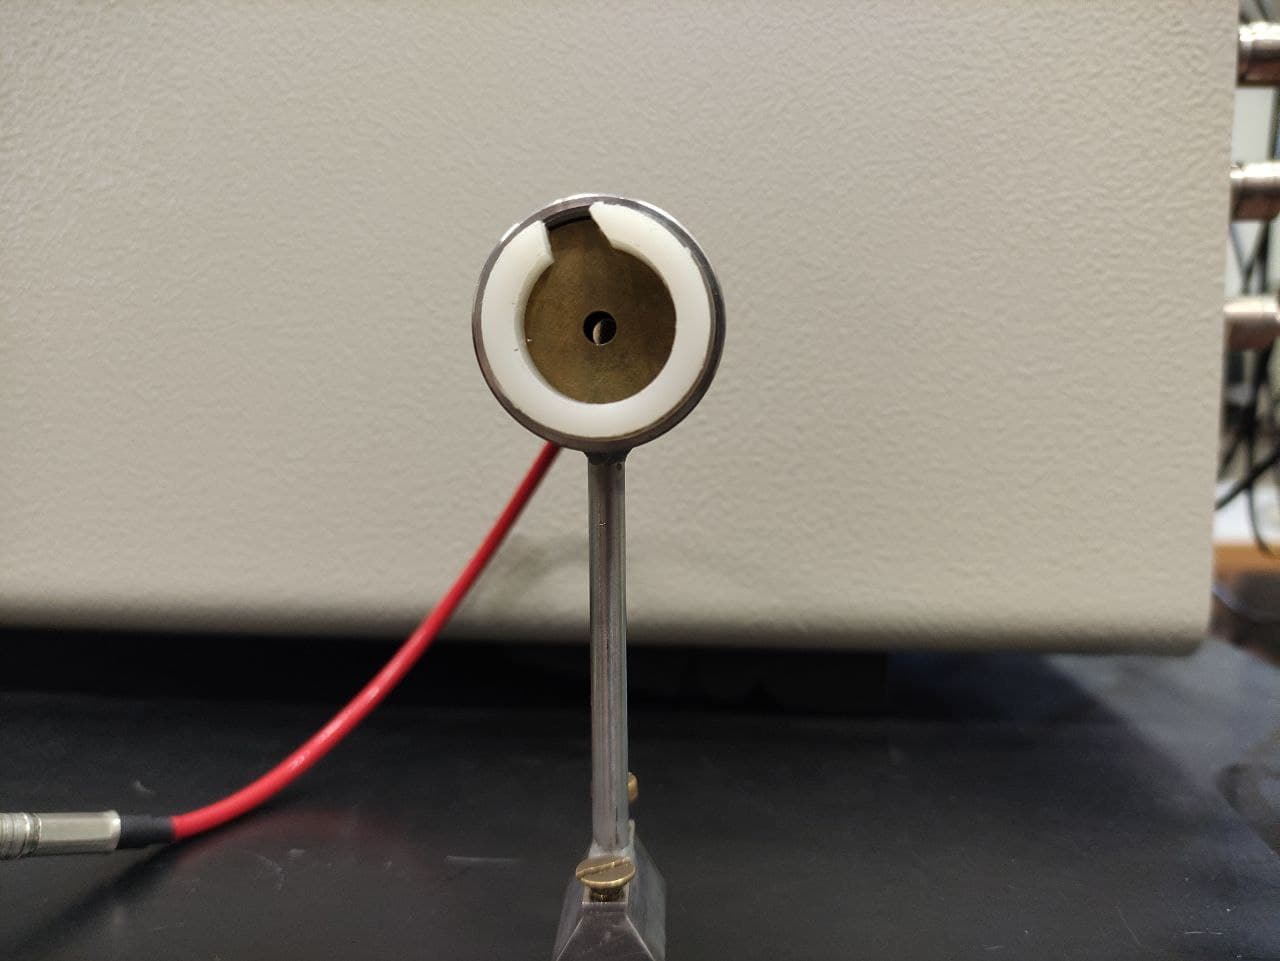
\includegraphics[width=\textwidth]{../sections/02/images/apparatus/SSB_support.jpg}%
            \label{fig:mechanical_ssb_support}%
        }%
    \end{minipage}%
    \hfill%
    \begin{minipage}[c]{0.33\linewidth}
        \vspace{0pt}
        \centering
        \subfloat[ALPIDE detector support]{%
            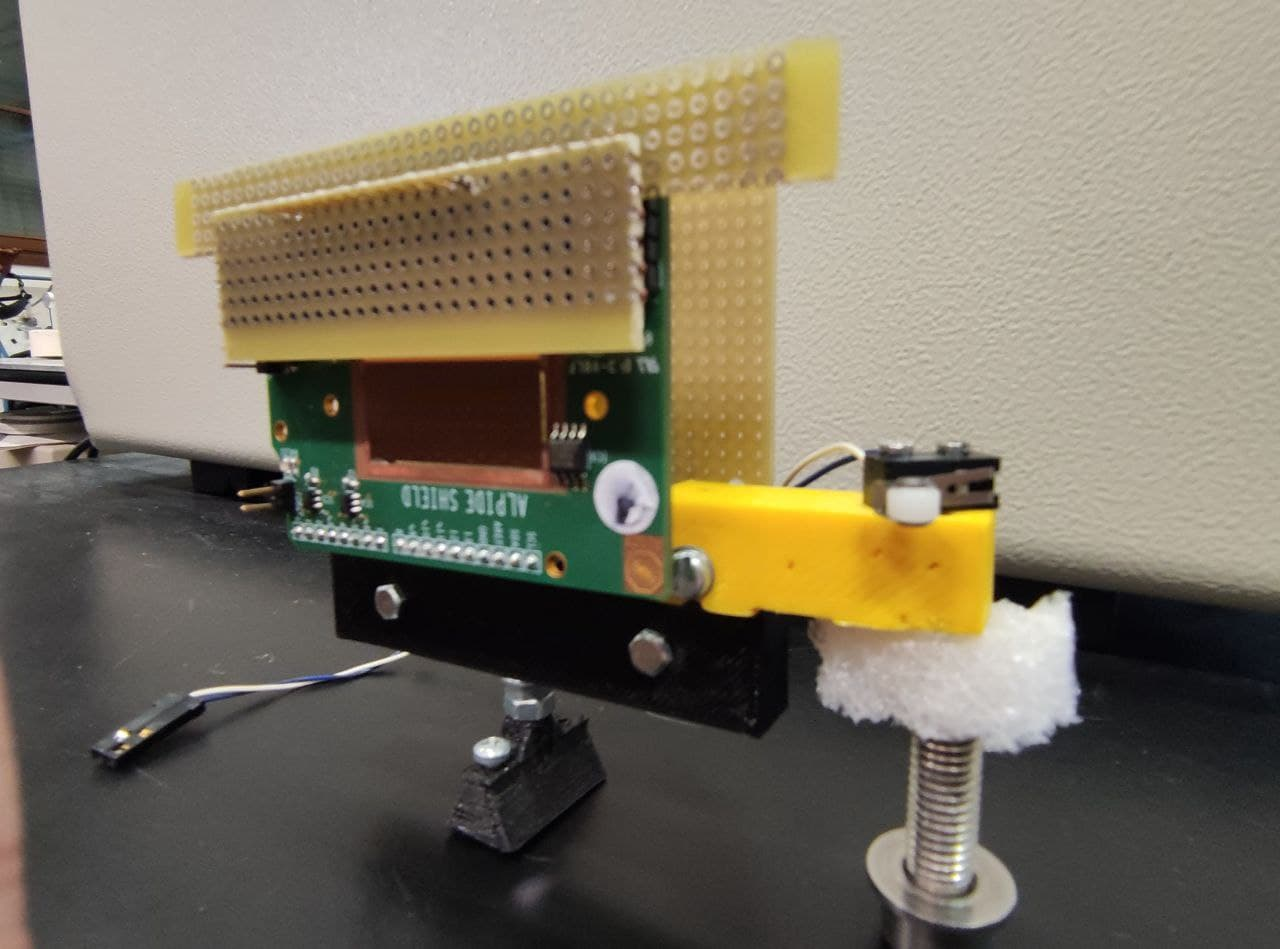
\includegraphics[width=\textwidth]{../sections/02/images/apparatus/ALPIDE_support.jpg}%
            \label{fig:mechanical_alpide_support}%
        }%
    \end{minipage}%
    \label{fig:mechanical_components}
    \caption{Components of the mechanical system of the experimental apparatus.}
\end{figure*}



\paragraph{Scattering foils}
For the measurements of \( \alpha \) particles scattering on a target, a set of thin foils of gold and tin are employed. These are characterised by a very small thickness, so they must be handled with great care when placing them in face of the source support, on which they are fixed through two screws. In particular, the specifics of the foils are given in \tabref{tab:mechanics_foil_specifics}.

\begin{table}[!h]
    \centering
    \begin{tabular}{cccc}
        \toprule
        \textbf{Foil material}  &   \textbf{\boldmath\( \rho_{\mathrm{sup}} \ \mathrm{[\mu g/cm^{2}]} \)} &   \textbf{\boldmath\( \rho \ \mathrm{[g/cm^{3}]} \)}  &   \textbf{\boldmath Thickness \( \mathrm{[\mu m]} \)}  \\
        \colrule
        gold    &   \( 325 \)   &   \( 19.32 \) &   \( 0.168 \) \\
        tin     &   \( 500 \)   &   \(  7.29 \) &   \( 0.686 \) \\
        \botrule
    \end{tabular}
    \caption{Specifics of the scattering foils employed for the experiment, in particular the superficial density, the volume density and the thickness are reported in columnar order.}
    \label{tab:mechanics_foil_specifics}
\end{table}



\subsection{Radioactive source}
% https://www.dfa.unipd.it/fileadmin/servtec/Sorgenti_polo_ott_2019_corretto.pdf
% https://www.ezag.com/fileadmin/user_upload/isotopes/isotopes/Isotrak/isotrak-pdf/Product_literature/EZIPL/EZIP_catalogue_reference_and_calibration_sources.pdf
% p. 67
% http://www.nucleide.org/DDEP_WG/Nuclides/Am-241_tables.pdf
The radioactive \( \alpha \) source employed for the experiment is schematized in \figref{fig:source_scheme_layers} \cite{source_ez}. The active material inside it is a layer of \( {}^{241}\mathrm{Am} \), covered by two consecutive thin layers of gold. These parts are inserted inside an aluminium support, whose diameter and length are about \( 12 \ \si{mm} \) and \( 79 \ \si{mm} \), respectively, and it is schematised in \figref{fig:source_scheme_cylinder}. A complete list of the relevant radiations and particles emitted by this source is given in \tabref{tab:source_emissions} \cite{source_ddep}. As we can see, we do not have only particles originated from \( \alpha \) decay, but also X and \( \gamma \) rays emissions. These are not a big deal for the SSB detector due to its working principles, but they constitute a relevant background for ALPIDE detector and special data analysis and statistical techniques should be employed, as we will see in the following Sections.

\begin{table}[h]
    \centering
    \begin{tabular}{ccc}
        \toprule
        \textbf{Emission}   &   \textbf{Energy [keV]} & \textbf{Weight}    \\
        \colrule
        \( \alpha \)    & \( 5485.56 \) &   \( 84.45 \) \\
        \( \alpha \)    & \( 5442.80 \) &   \( 13.23 \) \\
        \( \alpha \)    & \( 5388.25 \) &   \(  1.66 \) \\
        \colrule
        \( \gamma \)    & \( 59.5 \)    &   \( 35.92 \) \\
        X   &   \( 11.9 \divisionsymbol 22.2 \) &   \( 37.66 \) \\
        \botrule
    \end{tabular}
    \caption{Relevant emissions of the employed \( {}^{241}\mathrm{Am} \) source along with the corresponding energy. Concerning the weight, it should be intended as a probability of emission, for the \( \alpha \) decay mode, or as a number of photon emissions per \( 100 \) disintegrations, for the X and \( \gamma \) modes.}
    \label{tab:source_emissions}
\end{table}

Concerning the actual activity, it can be calculated knowing that in October 2019 it was \( \dot{N}(t_\mathrm{2019 \ Oct}) \approx 368.0 \ \si{kBq} \), as declared in \cite{source_dfa}:
\begin{equation}
    \dot{N}(t_{0})
    \approx
    \qty(\frac{1}{2})^{\frac{\Delta t}{t_{1/2}}}
    \quad .
    \label{eq:activity}
\end{equation}
Therefore, knowing the half-life of \( {}^{241}\mathrm{Am} \)\footnote{\( t_{1/2} = 432.14 \ \si{y}\).} and the temporal interval \( \Delta t \) from the last activity measurement to October 2020, we can approximate the source activity during the 3 months experimental measurements:
\begin{equation}
    \dot{N}(t_{0})
    \approx
    367.4 \ \si{kBq}
    \quad .
    \label{eq:source_actual_activity}
\end{equation}

\begin{figure*}[h]
    \begin{minipage}[c]{0.49\linewidth}
        \vspace{0pt}
        \centering
        \subfloat[Radioactive source layers]{
            \includestandalone[width=\textwidth, valign=c]{images/source/layers}
            \vphantom{\includestandalone[width=\textwidth, valign=c]{images/source/scheme}}
            \label{fig:source_scheme_layers}
        }
    \end{minipage}
    \hfill
    \begin{minipage}[c]{0.49\linewidth}
        \vspace{0pt}
        \centering
        \subfloat[Source scheme]{
            \includestandalone[width=\textwidth, valign=c]{images/source/scheme}
            \label{fig:source_scheme_cylinder}
        }
    \end{minipage}
    \label{fig:source_scheme}
    \caption{Radioactive source schemes of the layers covering the active material of \( {}^{241}\mathrm{Am} \) in \textbf{\ref{fig:source_scheme_layers}} and of the overall structure of the aluminium cylinder support in \textbf{\ref{fig:source_scheme_cylinder}}.}
\end{figure*}





\subsection{SSB detection system and electronics chain}
This part of the apparatus is composed of multiple modules. In this Subsection we briefly describe it briefly step by step. So, we have in logical order:
\begin{itemize}
    \item an ORTEC SSB Series A silicon detector, placed on an apposite support inside the vacuum chamber and interfaced to the external side of the chamber by a microdot-to-BNC connector;
    \item a Canberra 2003BT preamplifier, connected directly to the BNC interface in order to reduce the noise propagation along the electronics chain;
    \item a set of NIM modules for multiple purposes, including a polarizer, a shaping amplifier and a scaler for a raw real-time counting of the events detected by the silicon;
    \item lastly, a PicoScope 5000 oscilloscope working as a digitizer of the analogue signal coming from the amplifier. This block is connected to a computer which controls both the mechanical and the acquisition systems.
\end{itemize}


% http://nuchem.iucf.indiana.edu/SiSpecs/SBD_det_cat.pdf
\paragraph{ORTEC SSB silicon detector}
The first element of the chain is a so-called \textbf{partially depleted Silicon Surface Barrier (SSB)} detector, produced by ORTEC and with serial model A-035-025-300 \cite{ssb_detector}. A simple scheme of its structure is illustrated in \figref{fig:ssb_scheme}, where the values of the geometrical parameters are:
\begin{align}
    x &= 16.7 \ \si{mm} \label{eqn:ssb_x}   \\
    y &= 12.3 \ \si{mm} \label{eqn:ssb_y}   \\
    z &=  7.1 \ \si{mm} \label{eqn:ssb_z}   \\
    w &=  5.6 \ \si{mm} \label{eqn:ssb_w}   
\end{align}
Therefore, the active area of the detector is about \( 25 \ \si{mm^{2}} \). Concerning the rear part of the component, it has not a standard BNC connector, but a Microdot one. As given by the specifics of construction, the minimum depletion depth is \( 300 \ \si{\mu m} \), while the guaranteed maximum
resolution is approximately \( 35 \ \si{keV} \).

\begin{figure}[h]
    \includestandalone[width=0.4\textwidth]{\main/../sections/02/images/picoscope/ssb}
    \caption{ORTEC A-035-025-300 scheme with lateral and frontal views. The geometrical dimensions of the component are explicitly indicated and their values are given in EQS. \textbf{\ref{eqn:ssb_x}}-\textbf{\ref{eqn:ssb_w}}.}
    \label{fig:ssb_scheme}
\end{figure}


\paragraph{Canberra 2003BT preamplifier}
The Model 2003BT charge sensitive FET input preamplifier is employed due to its optimum performance with SSB detectors, as suggested by the user manual \cite{canberra_2003BT}. Operating as a charge to voltage converter, the unit accepts charge carriers produced in the detector during each absorption event. Then, the output provides a voltage in direct proportion to the collected charge.
For typical use with positively biased SSB detectors, an extremely linear energy output provides a positive polarity pulse which can be exploited for energy spectroscopy. The coincident timing output provides a negative polarity fast differentiated pulse, which allows to improve the resolution of the events in time.

The basic operation of the preamplifier is indicated in the functional schematic in \figref{fig:canberra_circuit}. The first stage acts as an operational integrator, which produces an output potential proportional to the accumulated charge on the feedback capacitor \( C_{\mathrm{f}} \).
The integrator drives the energy output directly. The timing output is derived from the integrator error signal through a pulse shaping network. Such an arrangement lowers the noise level and gives faster rise times.
To preserve pulse fidelity, the energy output is buffered through a series terminating resistor of \( 93 \ \si{\Omega} \).


\begin{figure}[h]
    \centering
    \includestandalone[width=0.75\textwidth]{\main/../sections/02/images/picoscope/canberra_circuit}
    \caption{Canberra 2003BT preamplifier circuit schematic, divided into a stage integrating the collected charge (proportional to energy output) and a final pulse shaper section for timing output.}
    \label{fig:canberra_circuit}
\end{figure}


\paragraph{NIM modules}
The next stage where an event signal detection goes through is the NIM modules rack. Going in order, the first one is a polarizer of the SSB detector, set at a \( \sim 100 \ \si{V} \) bias in order to be sure that the silicon wafer of the detector is sufficiently depleted but also not in the breakdown region. In fact, this would cause severe damages to the detector due to a rapid increase in the leakage currents.

The second NIM employed, whose input is directly connected to the preamplifier output, is the Canberra Model 2024 Fast Spectroscopy Amplifier \cite{canberra_2024}.
This near-Gaussian filter shaping is optimised to improve the pulse symmetry and to get minimum sensitivity to variations in detector rise time and maximum signal-to-noise ratio.
Unipolar shaping is achieved with one differentiator and two active filter integrators and offers six front panel switch selectable pulse shaping time constants.
% : \( 0.25 \), \( 0.5 \), \( 1 \), \( 2 \), \( 4 \) and \( 8 \ \si{\mu s} \).

The 2024 model includes also a Gated Integrator to reduce spectrum broadening at the shorter amplifier shaping time constants.
This component integrates the entire unipolar signal, providing a properly scaled linear output signal without the resolution degrading problems normally associated with fast amplifier shaping times and long detector charge-collection times.
% , an effect known as ballistic deficit.
% This effect is most pronounced for large volume detectors and with amplifier shaping times of less than \( 1 \ \si{\mu s} \).


\paragraph{PicoTech PicoScope 5244B digital oscilloscope}
This is the last part of the silicon detection system, employed as digitizer of the shaping amplifier output signal \cite{picoscope_5000}. It has memory storage of \( 256 \ \si{MS} \) (Mega-Samples) and it can be divided into more segments. The ensemble of the segments forms a block.

In the context of the experiment, the PicoScope is connected to a computer through USB cable and the operations done by the digitizer are the following, in chronological order:
\begin{itemize}
    \item the memory is firstly reset and zeroed, then it is divided into the number of segments required by the user;
    \item the trigger chosen by the user is set;
    \begin{itemize}[noitemsep,topsep=0pt,parsep=5pt,partopsep=0pt]%
        \item[\( \circ \)] every time the trigger is activated, the \( i^{\text{th}} \) segment is populated with the samples acquired;
        \item[\( \circ \)] after having filled the \( i^{\text{th}} \) segment, the \( (i+1)^{\text{th}} \) segment is filled...
        \item[\( \circ \)] ...and so on and so forth, until the last segment is filled;
    \end{itemize}
    \item PicoScope driver downloads the whole content of the memory on the computer and the cycle restarts.
\end{itemize}
It is important to remark that in these operations PicoScope sets the trigger once in a cycle, before starting to fill the segments. This operation constitutes a dead-time of about \( \sim 10 \ \si{\mu s} \). This is crucial when the expected rate of acquisition is high and in this case it is convenient to divide the memory block in a sufficient number of segments. On the other hand, when dealing with low rates, it becomes convenient to divide the memory into a single segment, so that every event constitutes a block. In fact, in this case the dead-time due to the reset of the trigger can be neglected.


\paragraph{Control software}
The software needed to control both the mechanical system and the PicoScope is written in Python, using the library ``wx'' for the handling of the GUI. After running the executable, the user can choose several commands in two sections, one for the motor and one for the PicoScope. In particular, it is possible to calibrate the motor, enable it and choose the step position. On PicoScope side, it is possible to change the acquisition parameters, such as the acquisition time, the trigger value in \( \si{mV} \), the number of segments, the events to acquire and the sample rate.




\subsection{ALPIDE detection system}
Also this detection system has a modular structure, but with a lower number of blocks with respect to the SSB detection system discussed above. In fact, ALPIDE detection system includes in logical order:
\begin{itemize}
    \item an ALPIDE chip mounted on the apposite support, placed inside the vacuum chamber and interfaced to an external FPGA;
    \item an Arty-A7 board, equipped with an Artix-7 FPGA;
    \item a NUC computer to provide the communications with the FPGA through the IPBus suite.
\end{itemize}


\paragraph{ALPIDE chip}
The ALPIDE sensor is developed for the ALICE Inner Tracking System (ITS). It is a \textbf{Monolithic Active Pixel Sensor (MAPS)}, where a collection diode and the readout electronics share the same monolithic silicon die, as it is schematised in \figref{fig:detection_alpide_frontend}.
This layout simplifies the connection between detectors and relative amplifiers. The detection area is arranged in a \( 1024 \times 512 \) pixel matrix with a \( 30 \times 15 \ \si{mm^2} \) form factor, where each pixel has its own analogue and digital chain, showed in \figref{fig:detection_alpide_pixel_chain}.


\begin{figure}[h]
    \centering
    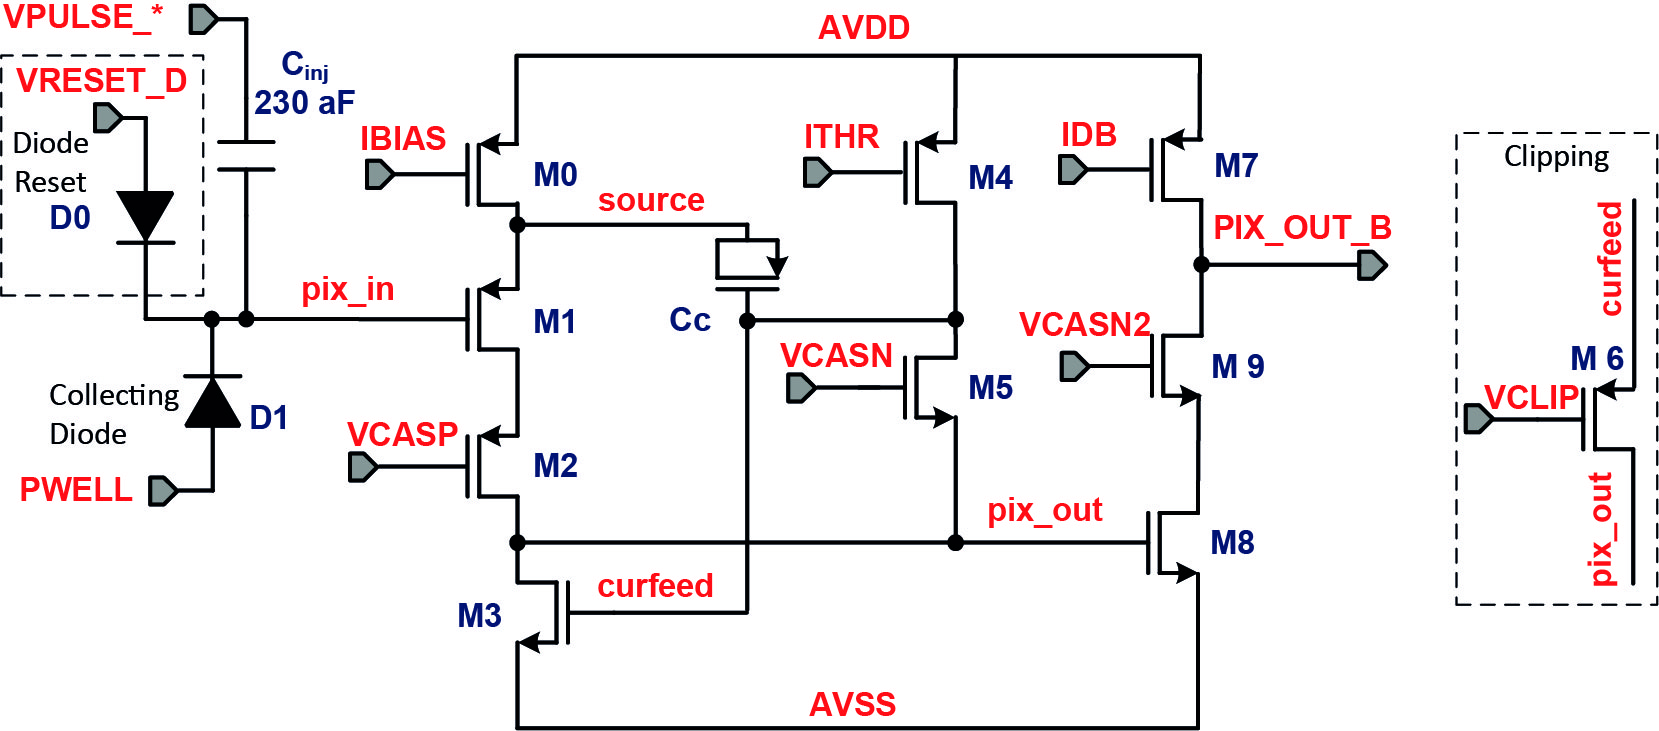
\includegraphics[width=0.85\textwidth]{../sections/02/images/alpide/FRONT-END.jpg}
    \caption{ALPIDE analogue frontend. D1 is the collection diode, M1 and M2 are a cascode preamplifier, M4 and M5 are the discriminator where the values of ITHR and VCASN  parameters can be modified to change the firing threshold value for \( n_{\mathrm{electrons}} \).}
    \label{fig:detection_alpide_frontend}
\end{figure}


\begin{figure}[h]
    \centering
    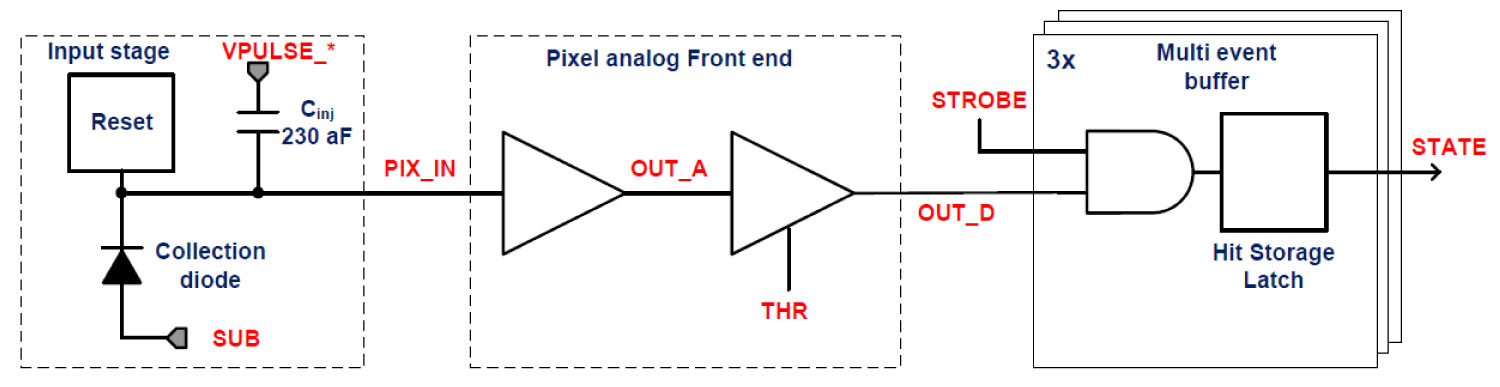
\includegraphics[width=0.85\textwidth]{../sections/02/images/alpide/Block_diagram.jpg}
    \caption{ALPIDE pixel signal chain. Some functionalities are highlighted, such as the so-called strobing, which acts as enable for storage latches, and the memory registers, 3 for each pixel.}
    \label{fig:detection_alpide_pixel_chain}
\end{figure}


The pixels are organised in double columns, which communicate to the control register through a priority encoder. The latter gives an address to each pixel and this is used to mask, pulse or read the state of a single pixel or a group of them through specific registers.

ALPIDE communicates with the DAQ system through two ports: the \textbf{CTRL port} (slower, \( 40 \ \si{Mbps} \)) and the \textbf{Data port} (faster, up to \( 1.2 \ \si{Gbps} \)). However, our PCB allows only the access to the CTRL port. This implies a limitation on the readout speed and so on the maximum event rate of acquisition.
Its protocol is described in the ALPIDE user manual \cite{Manual_ALP}: the FPGA sends a command for reading or writing, the address of target register and eventually the data to write. This has some similarities to the I$^2$C protocol.


\paragraph{Data acquisition firmware}
The FPGA board employed for the experiment is the XC7A35TICSG324-1L Arty A7 \cite{Arty_A7}. Its original firmware was developed in a previous work \cite{tesi_gabri} and it has been modified to fit our needs.
It consists in various state machines to decode (receiver functionality) and encode (transmitter functionality) the commands that come from or go to ALPIDE shield.
The system is timed by an internal clock of \( 40 \ \si{MHz} \), generated by a Mixed-Mode-Clock-Manager (MMCM)\footnote{Similar to a PLL (Phase Locked Loop), but with some advanced features} inside the FPGA. This clock reference is also propagated to ALPIDE detector.

The most important routines available in the framework are:
\begin{itemize}
    \item \textbf{initialisation} (\texttt{init}): it writes some specific registers to reset and set the chip in a predefined state;
    \item \textbf{read register} (\texttt{rr}): it reads a specific register;
    \item \textbf{write register} (\texttt{wr}): it writes a data on a specific register;
    \item \textbf{continuous readout} (\texttt{rope}): similar to the read register routine but it reads continuously two registers that are associated to the data stored in the ALPIDE data FIFO.
\end{itemize}
Several debug features are implemented in the FPGA as well, such as the status LEDs (``power on'', ``initialisation done'' and ``busy'' states) and error LEDs. Moreover, it is implemented with a suite that communicates with the PC, namely the IPBus suite \cite{IPBus}. This consists in various modules that connect the programmable logic available in the FPGA fabric to the ethernet controller, which sends and receives data from PC. The latter translates the ethernet packets exploiting the \texttt{$\mu$hal} Python and C++ library.

The connection to the ALPIDE shield is made of eight cables, showed in \figref{fig:detection_alpide_cables} and \figref{fig:detection_alpide_FPGA} and listed in \figref{tab:detection_alpide_cables}.


\begin{figure*}[h]
    \begin{minipage}[c]{0.33\linewidth}
        \vspace{0pt}
        \centering
        \subfloat[ALPIDE wiring]{%
            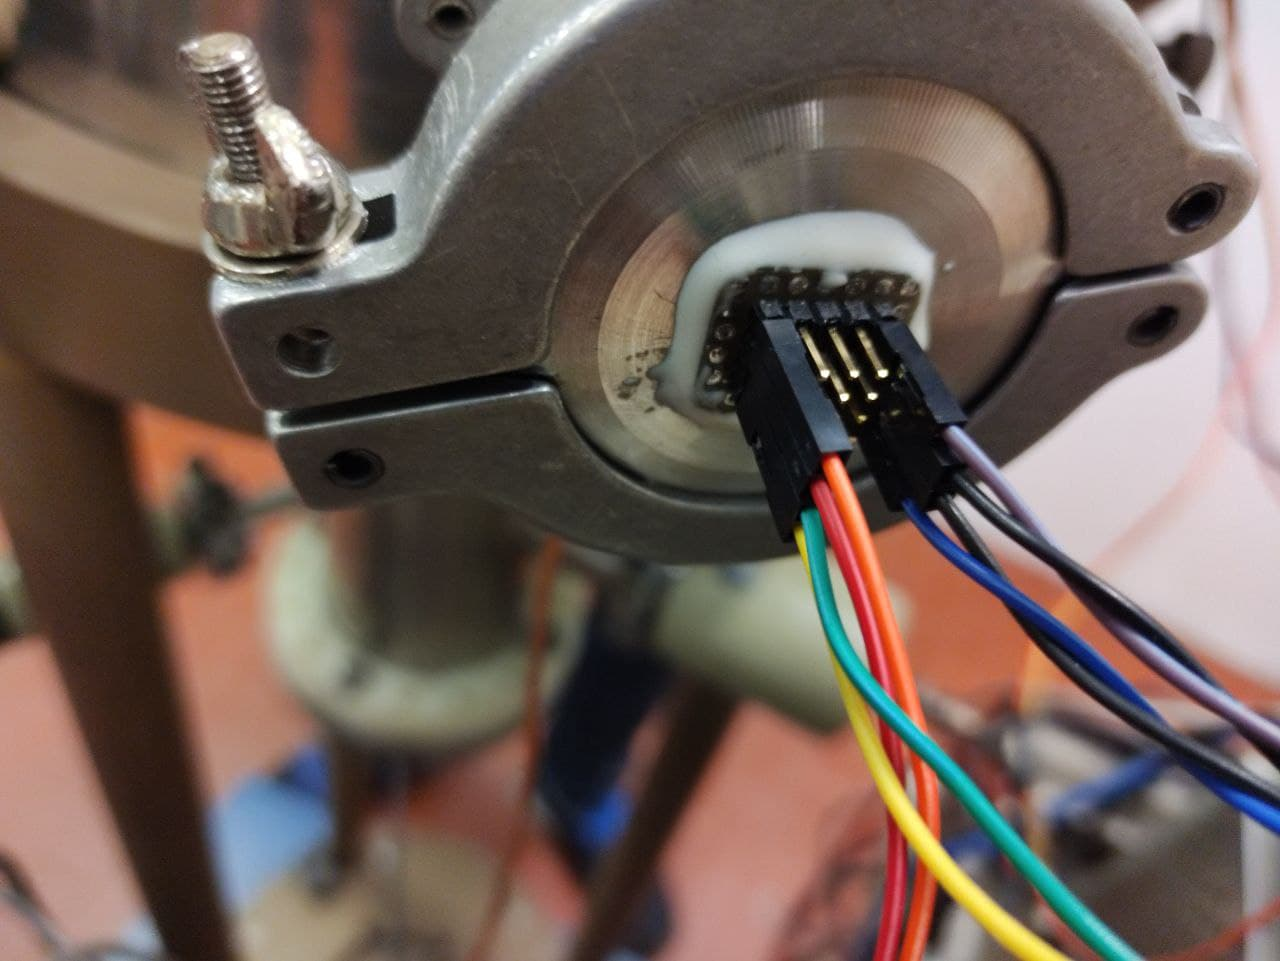
\includegraphics[width=\textwidth, valign=c]{../sections/02/images/apparatus/cables.jpg}%
            \label{fig:detection_alpide_cables}%
        }%
    \end{minipage}%
    \hfill%
    \begin{minipage}[c]{0.33\linewidth}
        \vspace{0pt}
        \centering
        \subfloat[FPGA wiring]{%
            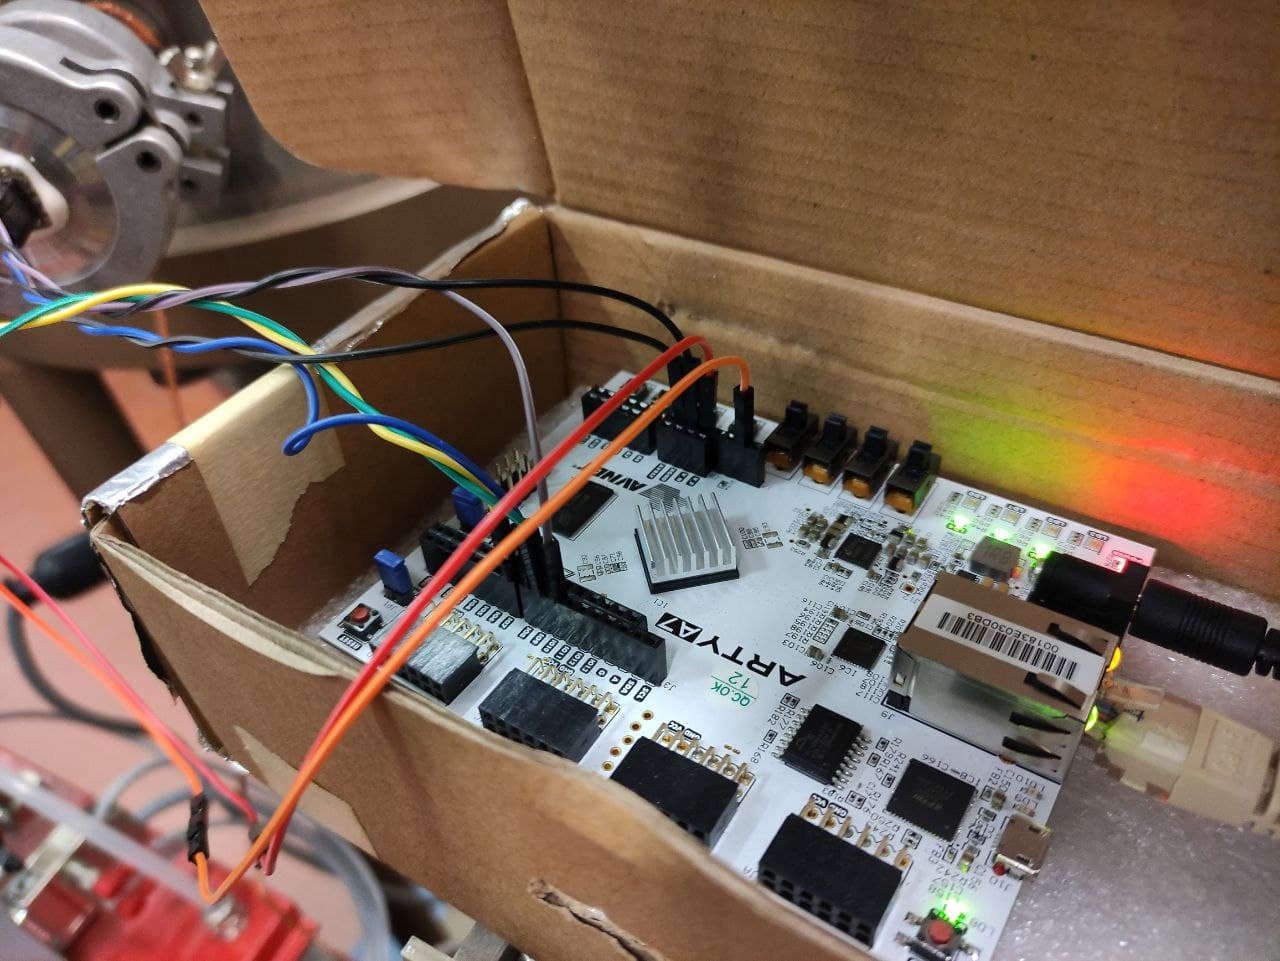
\includegraphics[width=\textwidth, valign=c]{../sections/02/images/apparatus/FPGA.jpg}%
            \label{fig:detection_alpide_FPGA}%
        }%
    \end{minipage}%
    \hfill%
    \begin{minipage}[c]{0.33\linewidth}
        \vspace{0pt}
        \centering
        \subfloat[List of cables]{
            \adjustbox{valign=c}{
            \begin{tabular}{ccc}
                \toprule
                \textbf{Cable}  &   \textbf{Symbol} &   \textbf{Colour} \\
                \colrule
                2 Grounds       &   \texttt{GND}        &   black   \\
                5V supply       &   \texttt{5V}         &   red     \\
                3.3V supply     &   \texttt{IO\_REF}    &   orange  \\
                ResetN          &   \texttt{RSTN}       &   yellow  \\
                Power enable    &   \texttt{P\_EN}      &   green   \\
                Clock           &   \texttt{DCLK}       &   brown   \\
                Control         &   \texttt{CTRL}       &   blue    \\
                \botrule
            \end{tabular}
            \label{tab:detection_alpide_cables}
            \vphantom{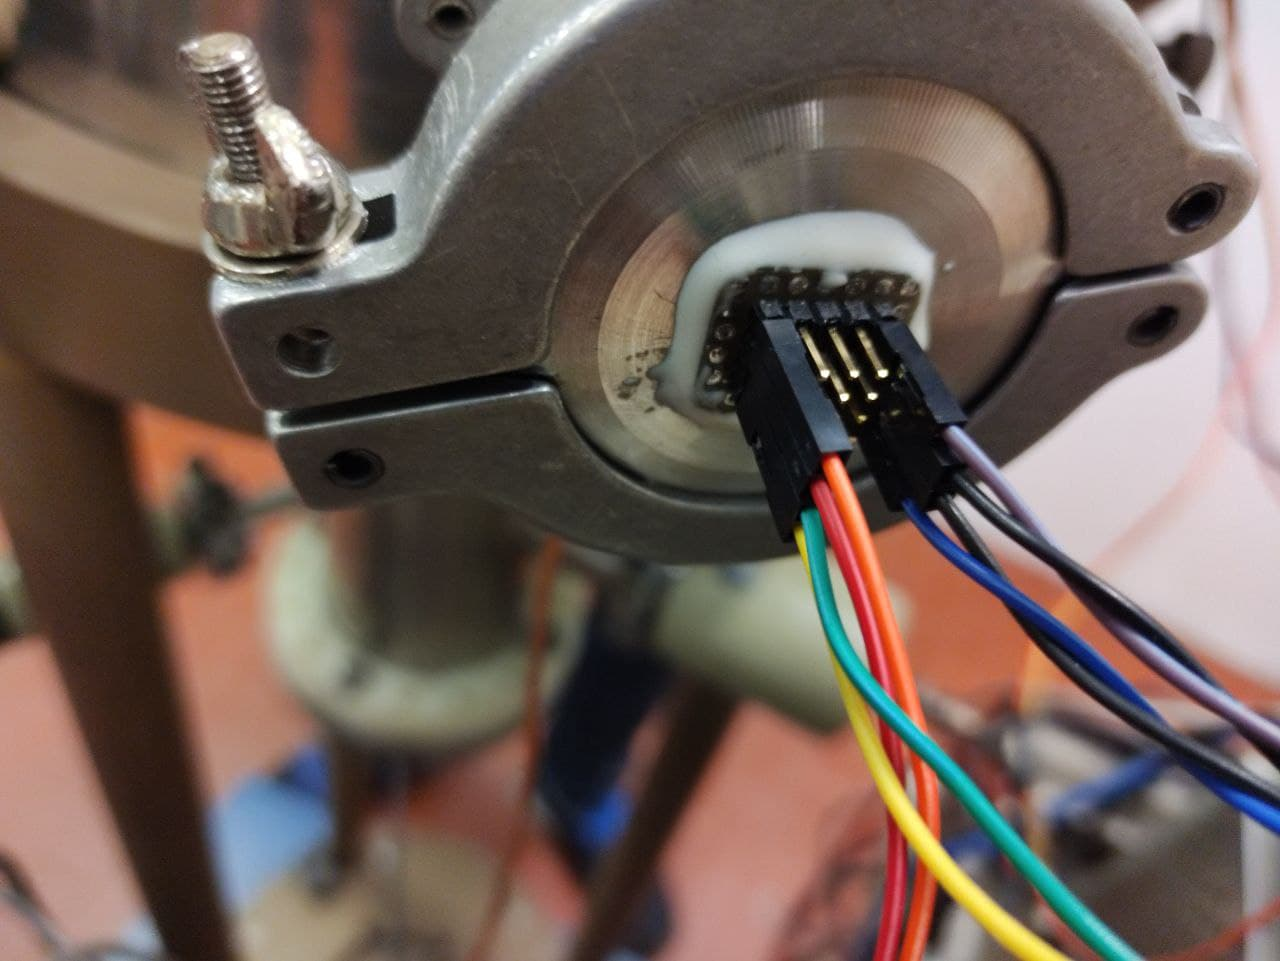
\includegraphics[width=\textwidth, valign=c]{../sections/02/images/apparatus/cables.jpg}}
            }
        }
    \end{minipage}%
    \label{figtab:detection_alpide_cables_}
    \caption{ALPIDE connections to the feedthrough in \textbf{\ref{fig:detection_alpide_cables}}, to the FPGA in \textbf{\ref{fig:detection_alpide_FPGA}} and list of their functionalities and corresponding colours in \textbf{\ref{tab:detection_alpide_cables}}.}
\end{figure*}


\paragraph{PC readout}
The readout and the ALPIDE control are performed by a Command Line Interface coded in Python 2.7. It allows to exploit some basic functionalities of the chip, such as power on/off ALPIDE, read/write registers and the most important one, namely the continuous readout.

ALPIDE has its own communication protocol and to read the data from the control port it necessary to extract the value from two specific registers, \texttt{DMU\_Data\_FIFO[15:0]} (\texttt{0x12}) and \texttt{DMU\_Data\_FIFO[23:16]} (\texttt{0x13}).
This read method implies a serious limitation on the effective throughput. In fact 218 clock cycles are necessary to read a single 24 bit data. This fact translates to an effective throughput of \( 4.404 \ \si{Mbps} \). On the other hand, the two high speed ports can reach a throughput of \( 320 \ \si{Mbps} \) (parallel) and \( 960 \ \si{Mbps} \) (serial with 8b/10b encoding). 

The effective throughput obtained in real data acquisition is \( 4.304 \ \si{Mbps} \). It is important to highlight in this context that the DMU (Data Management Unit) sends the acquired data in a packet format, described in the ALPIDE User Manual \cite{Manual_ALP}. Knowing these informations, it is possible to evaluate the time needed to read a single $\alpha$-cluster which has a mean area of about 30 pixels:
\begin{equation}
    r_{\mathrm{cluster}}
    =
    \sqrt{\frac{\mathrm{Area}_{\mathrm{cluster}}}{\pi}}
    \approx
    3 \ \si{px}
    \quad .
\end{equation}
This means that we have at least 3 double columns registers for event.
Enabling the compression of data in clusters (up to 8 adjacent pixels on a single 24bit data), we have a minimum of 6 data samples. Adding also the data formatting (Chip Header, Chip Trailer and 2 Region Header) we get a total of 10 data, which become 18 considering at least 2 additional noise pixels. These data samples correspond to a total of 3194 clock cycles (at 40 MHz) or about \( 100 \ \si{\mu s} \). So, this detection system can stand a maximum theoretical rate of \( 10^{4} \ \si{ev/s} \).
However, this limit is lowered by the drawbacks of using the slow port: the ALPIDE FIFO overflow. In fact, the memory has a depth of 64 locations, so there is a limit of about 3 $\alpha$-clusters stored before the assertion of a critical readout flag.


\subsection{Internal network}
In order to produce statistically significant results, long acquisition times are required.
This fact, alongside with the necessity of monitoring the system during acquisition, makes necessary the possibility of controlling the whole setup from a remote location. To do this, we employ a switch to create a Local Area Network, which allows us to connect and control the two detectors and the step motor through an \texttt{ssh} connection. In \figref{fig:LANfoto} the network setup is showed, while in  \tabref{tab:ipaddr} its nodes are listed.


\begin{figure*}[h]
    \begin{minipage}[c]{0.49\linewidth}
        \vspace{0pt}
        \centering
        \subfloat[LAN Network Diagram]{
            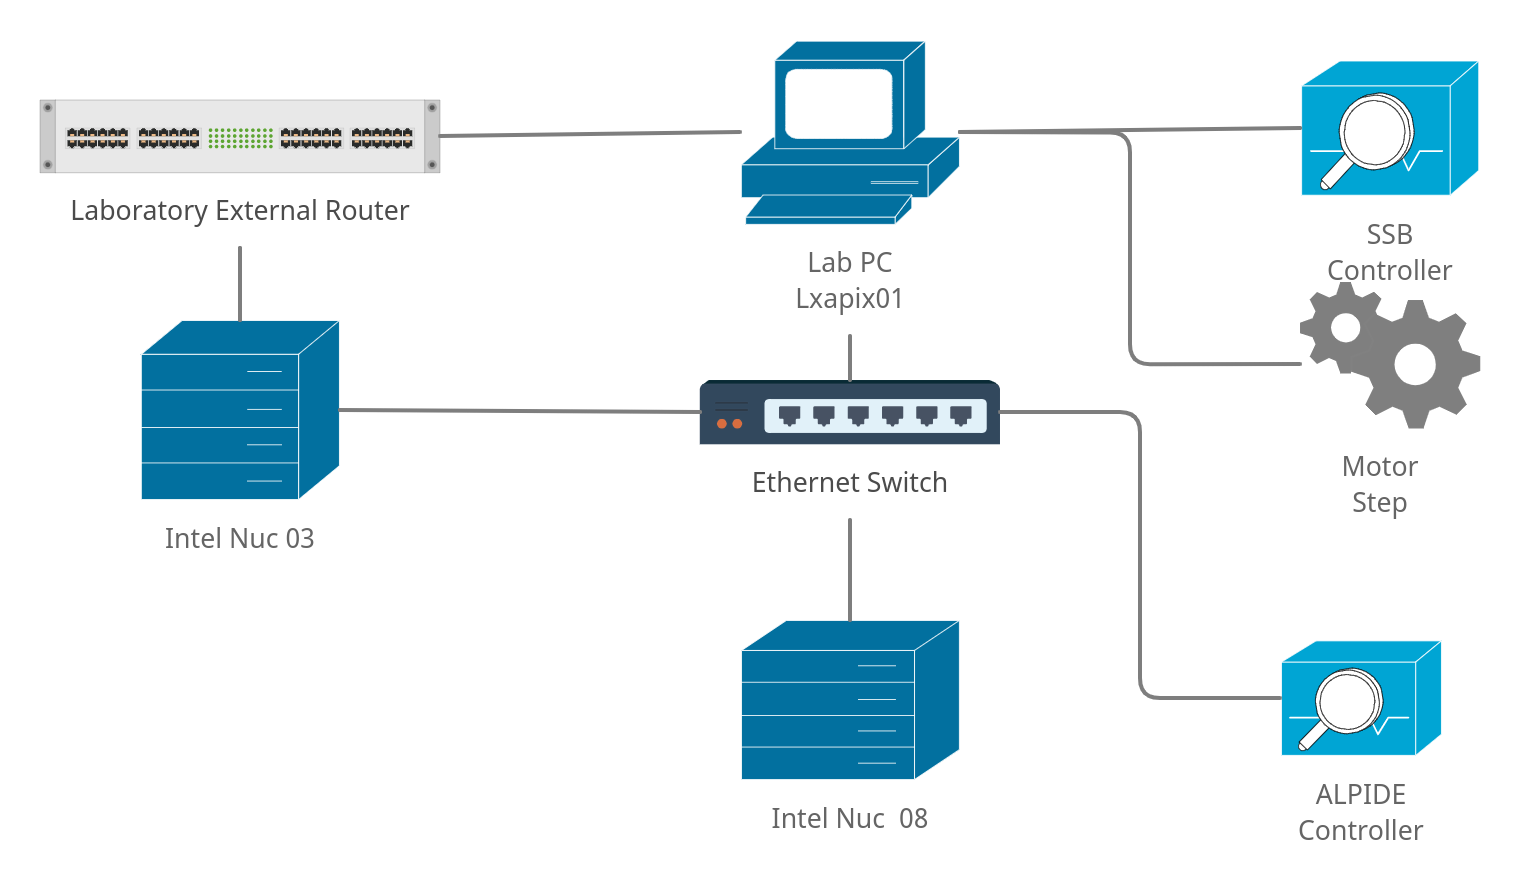
\includegraphics[width=1.0\linewidth, valign=c]{../sections/02/images/LabNetowrk.png}
            \label{fig:LANfoto}
        }
    \end{minipage}%
    \hfill%
    \begin{minipage}[c]{0.49\linewidth}
        \vspace{0pt}
        \centering
        \subfloat[IP Addresses of the LAN nodes]{
            \adjustbox{valign=c}{
                \begin{tabular}{cc}
                    \toprule
                    \textbf{IP}  &     \textbf{Device} \\
                    \colrule
                    \texttt{10.10.10.2}    &   Lab PC \texttt{laxpix01}          \\
                    \texttt{10.10.10.20}   &   Intel \texttt{NUC 08} Mini PC    \\
                    \texttt{10.10.10.30}   &   Intel \texttt{NUC 03} Mini PC    \\
                    \texttt{10.10.10.100}  &   ALPIDE Controller      \\
                    \botrule
                \end{tabular}
                \label{tab:ipaddr}
            }
            \vphantom{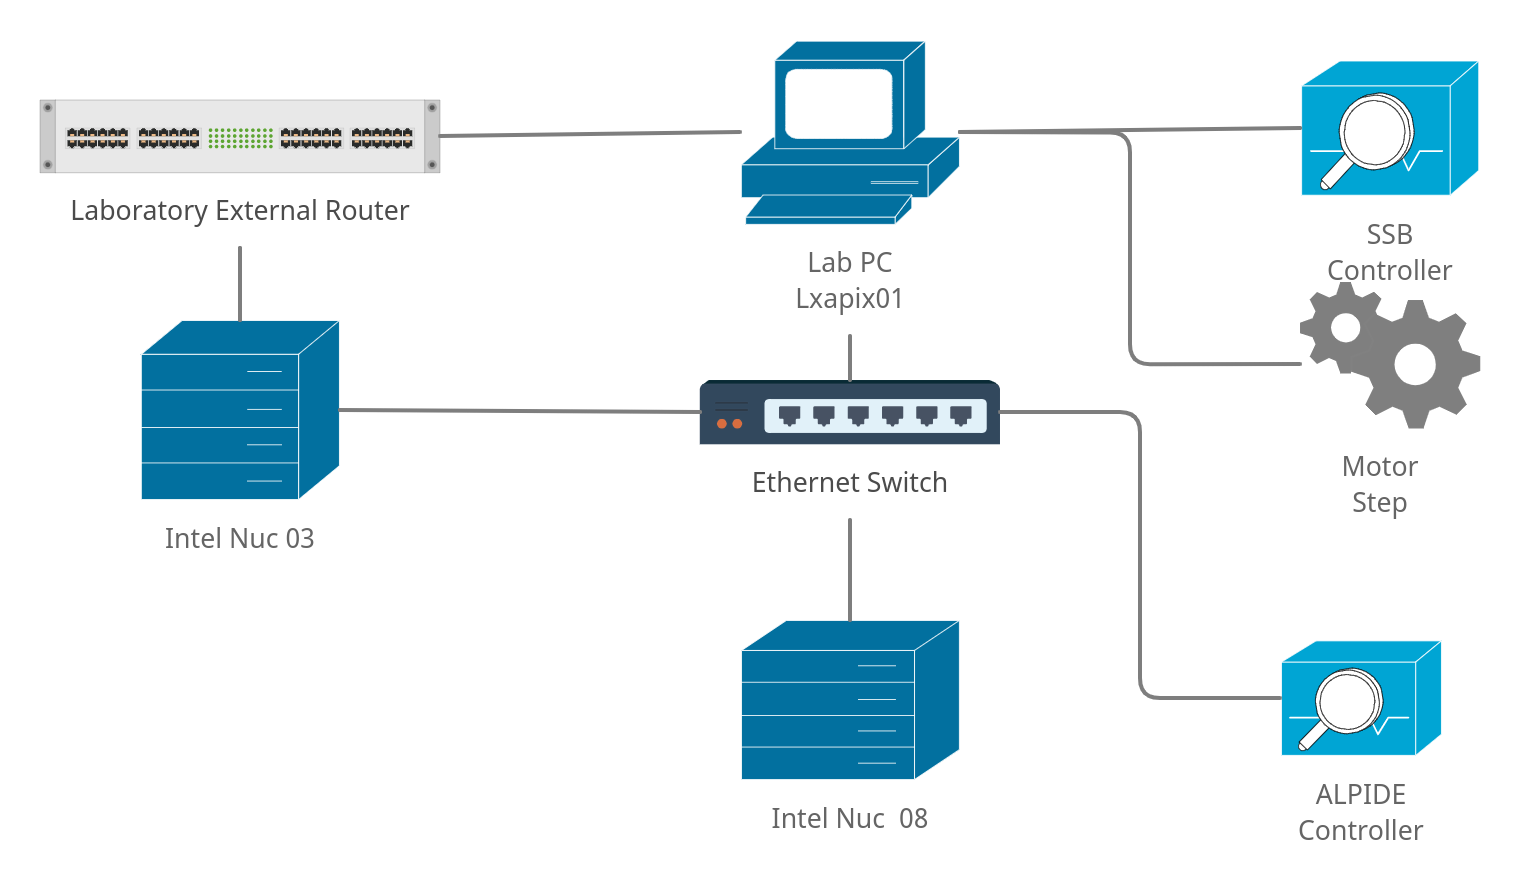
\includegraphics[width=1.0\linewidth, valign=c]{../sections/02/images/LabNetowrk.png}}
        }
    \end{minipage}
    \caption{Network diagram for the LAN setup in \textbf{\ref{fig:LANfoto}}, where the main components for the remote monitoring are explicitly remarked. In \textbf{\ref{tab:ipaddr}}, a list of the IP addresses corresponding to the main devices.}
    \label{figtab:LAN}
\end{figure*}

As we can see from \tabref{tab:ipaddr}, the step motor and the Arduino controller are not present, since these are controlled from the laboratory PC via USB connection. So, a total number of three computers is present inside the network: one for motor and SSB detector control, another one for ALPIDE detector control, and the last one for simultaneous control of both the acquisition systems.

\end{document}
